\documentclass[12pt]{article}

%% Language and font encodings
\usepackage[english]{babel}
\usepackage[utf8x]{inputenc}
\usepackage[T1]{fontenc}
%% Sets page size and margins
\usepackage[a4paper,top=2cm,bottom=2cm,left=3cm,right=3cm,marginparwidth=1.75cm]{geometry}

%% Useful packages
\usepackage{amsmath}
\usepackage{graphicx}
\usepackage{multirow}
\usepackage[ruled, vlined]{algorithm2e}
\usepackage[colorinlistoftodos]{todonotes}
\usepackage[colorlinks=true, allcolors=blue]{hyperref}
\usepackage{float}
\usepackage{url}
\title{Spring 2018\\  ECE563 Large Course Project}
\author{Charitha Saumya Gusthinna Waduge (cgusthin@purdue.edu) \\ Ehab Mohammad Ghabashneh (eghabash@purdue.edu)}

\begin{document}
\maketitle
\section{Overall Strategy}
\subsection{OpenMP implementation}
\label{omp-impl}
This section will discuss a lock free strategy for implementing the Map-Reduce programming model that we used for out OpenMP version. Map-Reduce has four main steps. First, reading input files, and divide the input files into separate lines. Second, map each word in each line using {\em DJB2}~\cite{djb2} hash function. Third, reducing words from different input files. Last, writing the word count. 

Each reader will take a set of input files and fill them into separate queues. Thus, each file has its own linked-list queue. Reader will read the file line by line; each line is a node in a linked-list queue. Each queue linked-list has head and tail. While reader uses tail to put data (line) on the queue, mapper will use the head to get data (line) from the queue. This queue linked-list has a synchronization problem, which happens if the queue has one node left{\em (head = tail)} at any moment. If the mapper gets to the head first, it will take the line of data, and head will be NULL. Then, the reader will add new line to the tail. But head is not linked to the linked-list anymore. To solve this issue, the mapper cannot take data from the head if the {\em head->next==NULL}. Unless, reader has finished reading the whole input file. 

Each mapper will map a set of input files. As discussed, each mapper will use the heads of queues for couple of files to map words using {\em DJB2} hash function; creating a hash table for each file. Thus, {\em Read\_Map} operation will convert each file into a hash table that contains the words of the file and the count of appearance for each word. Each entry in a hash table is a node in a linked-list. In case two words have the same hash value, the new word will be added to the head of the linked-list.

Each reducer will take a specific range of the hash tables. For example, if the number of files is 3, and hash table size is 1000; with four reducers, reducer 1 will take indices from 0-249 of hash table 1,2 and 3. Reducer 2 will take indices 250-499 of hash table 1,2 and 3, and so on. For each entry in a hash table, the reducer will look for it in the other hash tables; it will delete the entry wherever it is found. Each time reducer reduces a word, it will write it on a file. Thus, each reducer will create a file that contains the words it reduced.
\subsection{MPI implementation}
In the MPI implementation we split the files in {\em RawText } directory among the available MPI processes. The distribution of files is done by a master process ( process $0$).
Master process read all the filenames in the input directory and stores them in a list. Then later sends $m$  number of files to each worker process in a round robin fashion as long as the file
list is not empty. If the file list is empty master sends a special {\em ``all done!''} message to all worker processes. Each worker process keeps receiving files in to its local file list until
it receives the {\em``all done!''} message. After all the files are received, a worker run its own instance of OpenMP map reduce which is described in section~\ref{omp-impl}. The results of the
local map reduce is written in to $P$ number of files where $P$ is the number of worker processes. 

\noindent \textbf{Sender Thread} : In the next step each worker initiate a sender thread and receiver thread. Sender threads job is
to send the local result to the worker who is responsible for the global reduction. For example if process $P1$ is responsible for counting the word {\em ``always''} all the other worker processes send their
local counts of that word to $P1$ and $P1$ does the final reduction. In our implementation the word count hash table is split among the processes uniformly i.e. if the hash table size is $M$ each worker gets 
to reduce $M/P$ of words where $P$ is the number of workers. If the sender is done with a local result that needs to be sent to a specific worker it will send a special {\em ``end of file''} message. This
lets the receiving end know that it received the complete result from this sender. 

\noindent \textbf{Receiver Thread} : The receiver thread does the final reduction on the set of words assigned it. Receiver keeps receiving local results from all the other processes until it 
receives the {\em ``end of file''} messages from all 
other workers. At the end receiver writes it final reduction result to a file. Therefore at the end there will be $P$ files containing the final result each corresponding to specific portion of the word 
count hash table. 

\noindent \textbf{Communication Strategy} : We used a fairly simple communication strategy for the whole MPI implementation. For the file name distribution, since only the master process is sending and all others are 
receiving its straight forward to use {\em MPI\_Recv}'s at the receiving end. But things get little complicated in the reduction step because every process need to send different data to every other process. This makes 
it difficult to know in what order the messages will be received by a given process. We solved this problem by using {\em MPI\_Recv}'s with {\em MPI\_ANY\_SOURCE} as the source and {\em MPI\_Status} tells us who actually sent 
the message.
\section{Evaluation of OpenMP version}
\subsection{Reader}
The reader performance is not as promised which is due to excessive use of {\em malloc}. {\em malloc} function is thread-safe which means all threads will be fighting on it due to synchronization on it. Figure~\ref{fig:reader} shows how reader performance declines with increasing the number of threads. 
\begin{figure}[H]
\centering
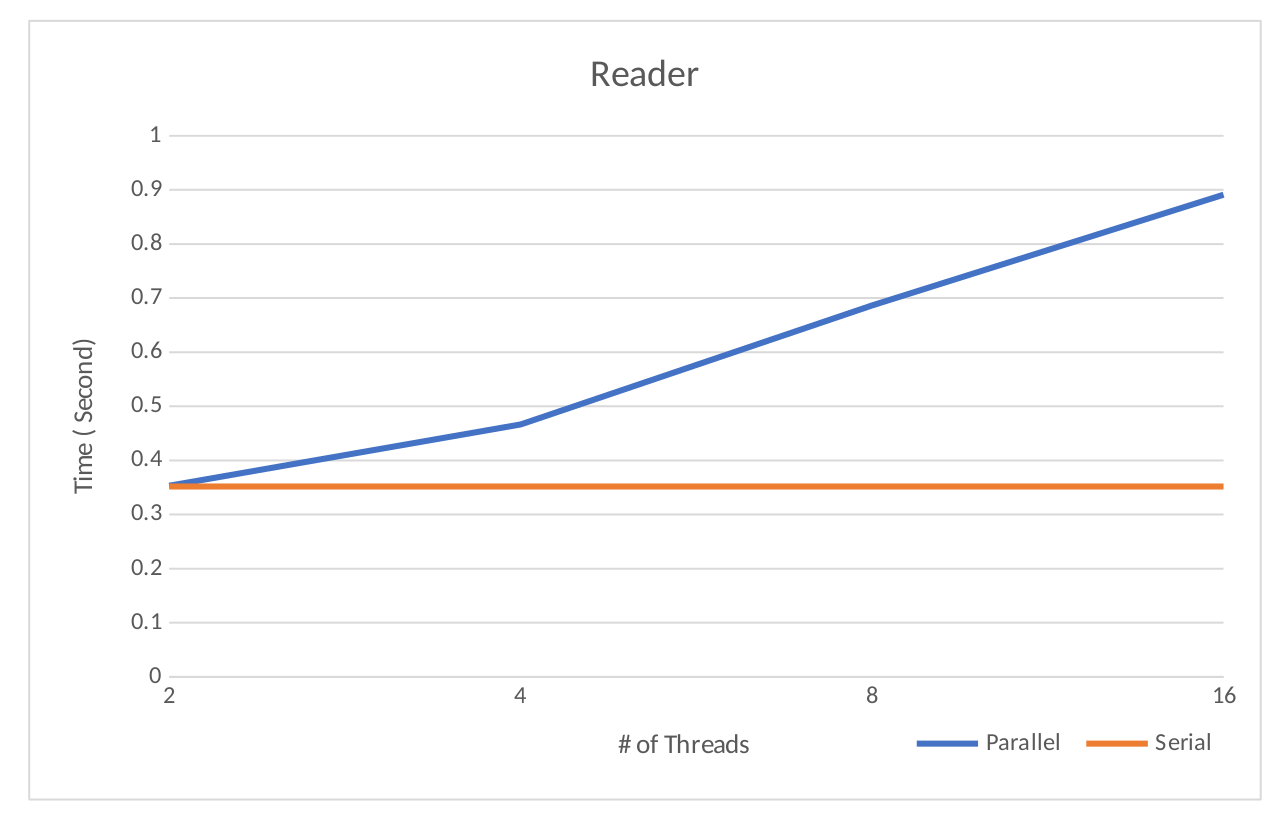
\includegraphics[width=0.7\textwidth]{fig/reader.png}
\caption{Performance of Readers \label{fig:reader}}
\end{figure}

\subsection{Mapper}
The performance of mappers increases as the number of threads increases. Figure~\ref{fig:mapper} shows how the performance of mappers increases, reaching the peak at 8 threads. Then, it starts declining because the increase in the overhead of threads beats the decrease in the parallel time.
\begin{figure}[H]
\centering
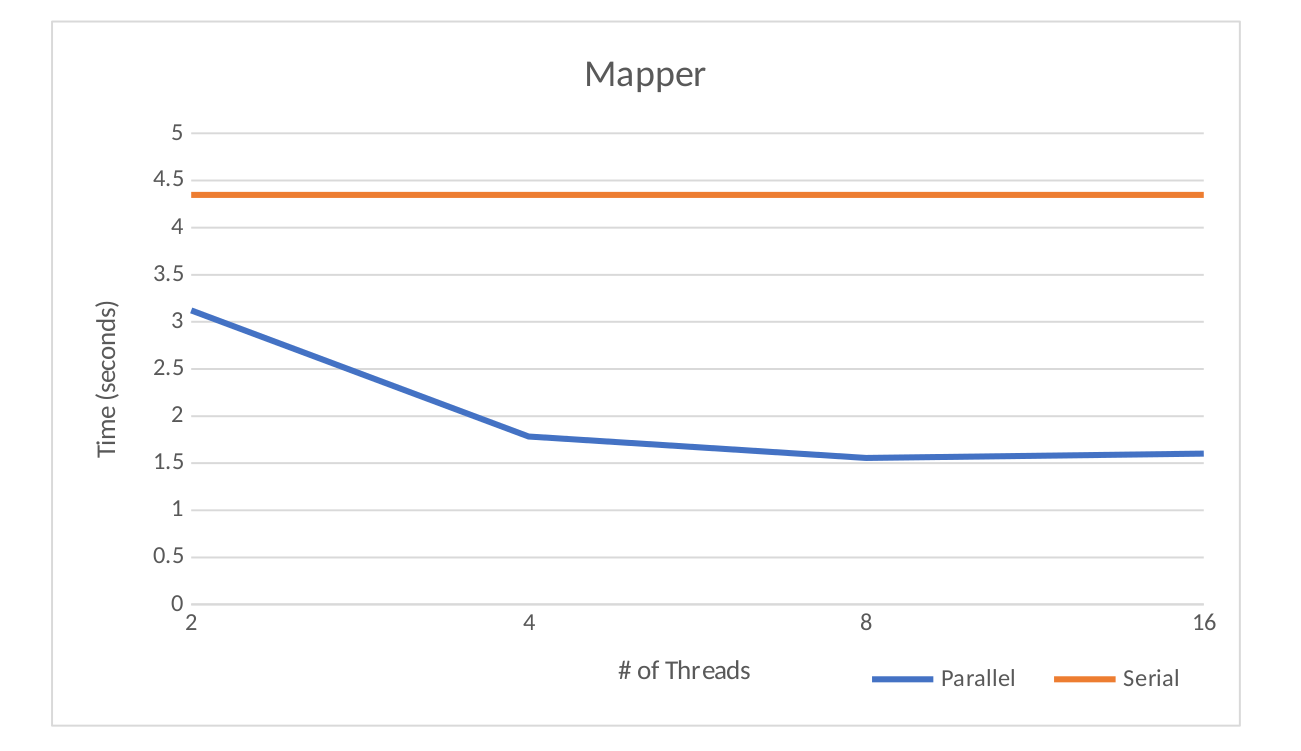
\includegraphics[width=0.7\textwidth]{fig/mapper.png}
\caption{Performance of Mappers \label{fig:mapper}}
\end{figure}

\subsection{Performance of Readers and Mappers}
The mappers and readers work simultaneously in our design. So, even the performance of readers is not as promised but it will have a small effect on the overall performance. Mappers take more time than the readers, since each mapper has to split the line into words, and hash each word. While reader will only read the file line by line.  Thus, fighting on {\em malloc } among readers will not worsen the performance of {\em Read\_Map} operations. Figure~\ref{fig:readmap} shows the performance of {\em Read\_Map} operation.
\begin{figure}[H]
\centering
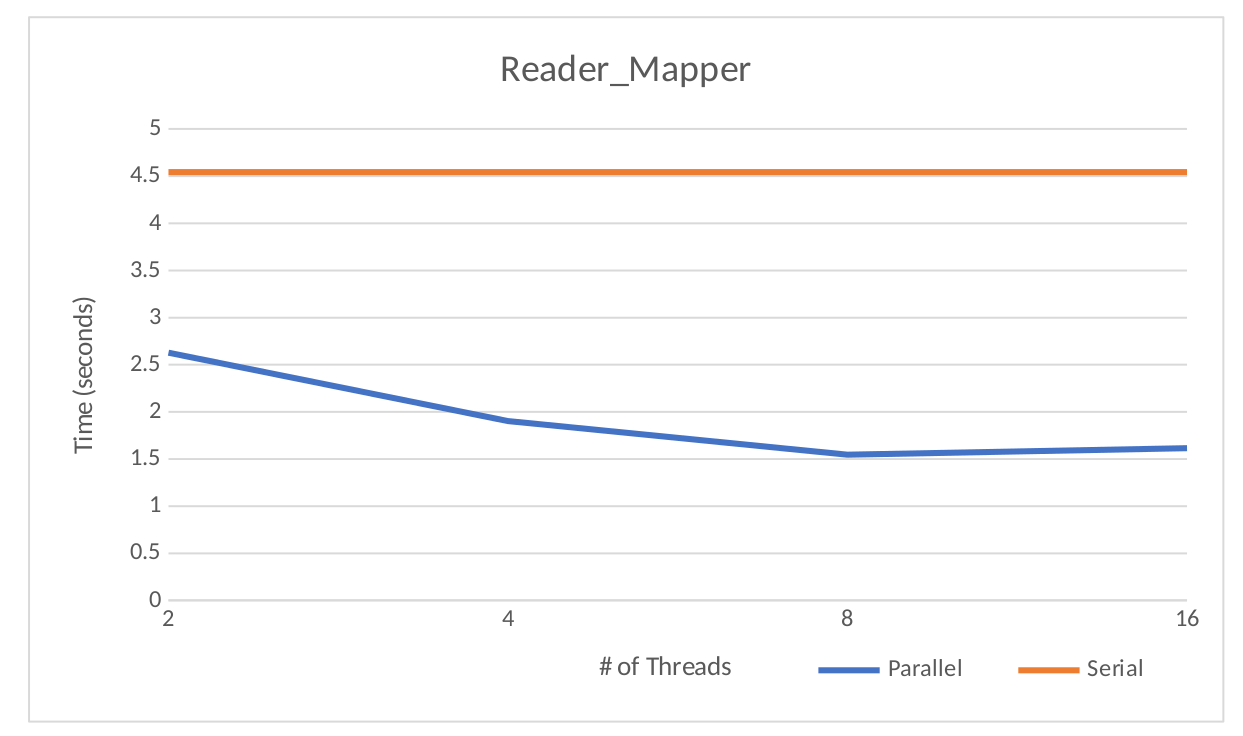
\includegraphics[width=0.7\textwidth]{fig/reader_mapper.png}
\caption{Performance of Readers and Mappers \label{fig:readmap}}
\end{figure}

\subsection{Reducer}
The performance of reducers increases along with the increase in the number of threads. Figure~\ref{fig:reducer} shows the performance results.
\begin{figure}[H]
\centering
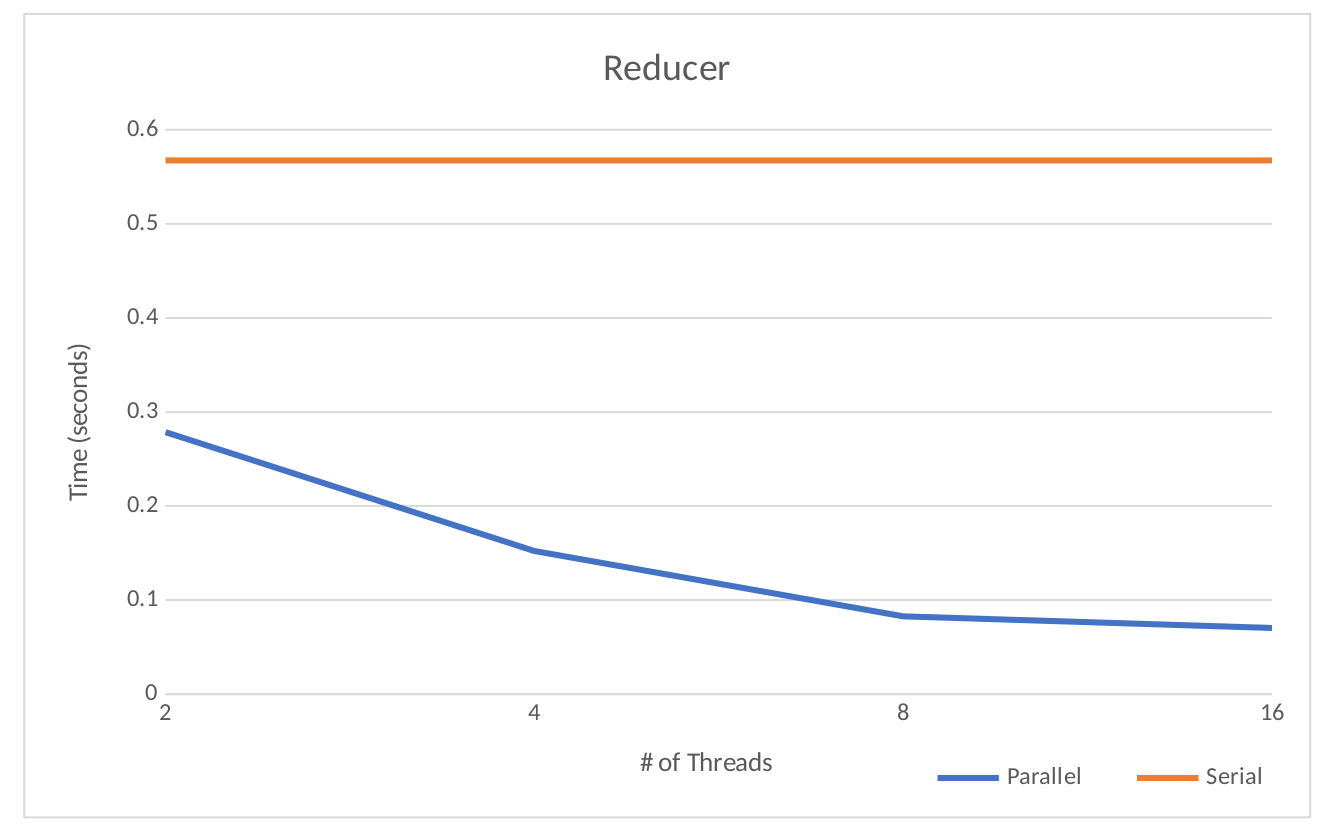
\includegraphics[width=0.7\textwidth]{fig/reducer.png}
\caption{Performance of Readers and Mappers \label{fig:reducer}}
\end{figure}

\subsection{Overall Performance}
Figure~\ref{fig:overall} shows the overall performance of lock free OpenMP version. Results show the execution time improvement, but the improvement start declining with using more than 8 threads because of the aforementioned overhead issue. 
Table~\ref{omp-tbl} shows the speed up, efficiency, and Karp-Flatt Metric.

\begin{figure}[H]
\centering
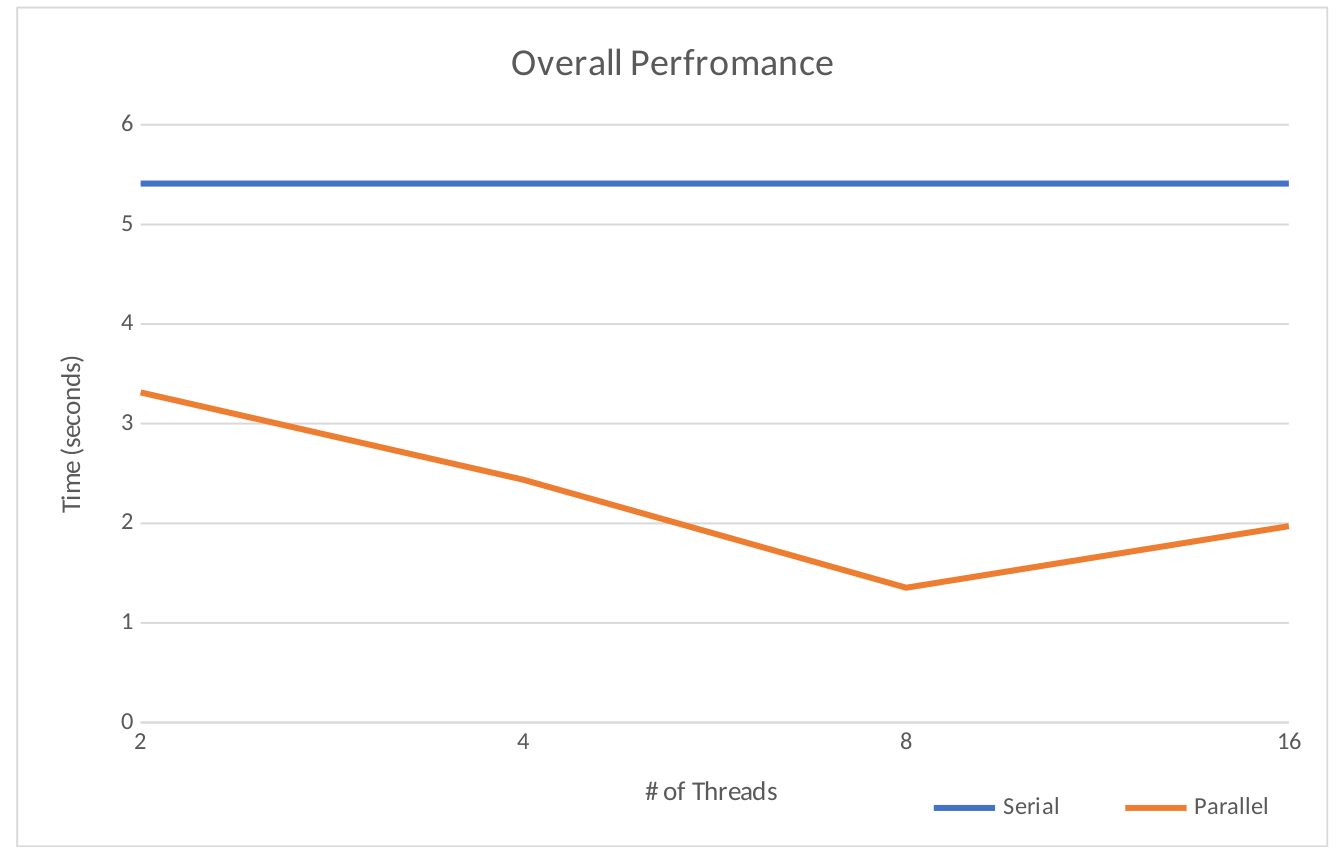
\includegraphics[width=0.7\textwidth]{fig/overall.png}
\caption{Overall Performance \label{fig:overall}}
\end{figure}

\begin{table*}[ht]
\centering
%\resizebox{\columnwidth}{!}{
\begin{tabular}{|l|l|l|l|}
\hline
    No of threads & Speedup & Karp-Flatt Metric($e$) & Efficiency \\ \hline
    2  & 1.63 & 0.22 & 0.82 \\ \hline
    4  & 2.25 & 0.26 & 0.56  \\ \hline
    8  & 4.04 & 0.14 & 0.51\\ \hline
    16 & 2.76 & 0.31 & 0.17 \\ \hline
\end{tabular}
%}
    \caption{Speedup, Efficiency and Karp-Flatt metric for OpenMP version \label{omp-tbl}}
\end{table*}

\section{Evaluation of MPI version}
For evaluating the performance of our implementation we ran it on the scholar cluster with 2, 4, 8 and 16 nodes. The number of thread available on each node was
set to 8. In order to give the program a large enough input size we repeated the files in {\em RawText} directory 10 times. Same input was used for all the runs. 
\subsection{Speedup}
For calculating the speedup we used a sequential version of the word-count map reduce which does not have any parallelism i.e. it uses a single thread for
all the work. Results are shown in table~\ref{speedup-tbl}. We achieved the best speedup for 8 nodes. However speedup started to decrease after 8 nodes due
to the increasing parallel overheads.
\begin{table*}[ht]
\centering
%\resizebox{\columnwidth}{!}{
\begin{tabular}{|l|l|l|l|}
\hline
 No of Workers & Parallel time  & Speedup \\ \hline
 2  & 2.5178 & 3.3044 \\ \hline
 4  & 1.9435 & 4.2808  \\ \hline
 8  & 1.9179 & 4.3379   \\ \hline
 16 & 2.5455 & 3.2684   \\ \hline
\end{tabular}
%}
    \caption{Running time (in seconds) and speedups for MPI version \label{speedup-tbl}}
\end{table*}
\subsection{Efficiency}
For efficiency calculations we computed the speedups again compared to a OpenMP version run on single node i.e. speedup is achieved using distributed memory 
parallelism whereas shared memory parallelism is present in both single and multi-node versions. This is because we got efficiencies values over 1 when they were calculated using MPI version and plain sequential version of the 
algorithm. Computed efficiency values are shown in table~\ref{eff-tbl}. We got the highest efficiency for 2 nodes and the efficiency quickly diminished when the 
no of nodes is increased.
\begin{table*}[ht]
\centering
%\resizebox{\columnwidth}{!}{
\begin{tabular}{|l|l|l|l|}
\hline
 No of Workers & Single node speedup  & Efficiency \\ \hline
    2  & 1.4714 & 73.57\%   \\ \hline
    4  &  1.9061 & 47.65\% \\ \hline
    8  & 1.9316 & 24.14\% \\ \hline
    16 &  1.4554 & 9.10\% \\ \hline
\end{tabular}
%}
\caption{Efficiency of the MPI version \label{eff-tbl}}
\end{table*}

\subsection{Karp-Flatt Analysis}
Karp-Flatt analysis was performed using the speedups shown in table~\ref{eff-tbl} and figure~\ref{evals} shows the variation of Karp-Flatt
metric. It is clear that sequential fraction of the parallel execution is increasing rapidly in our implementation which explains the decreasing
efficiencies and speedups. This is due to the increasing overheads due to OpenMP threads fighting over {\em malloc}, MPI communication overhead and
dumping partial word-counts to files.

\begin{figure}[H]
\centering
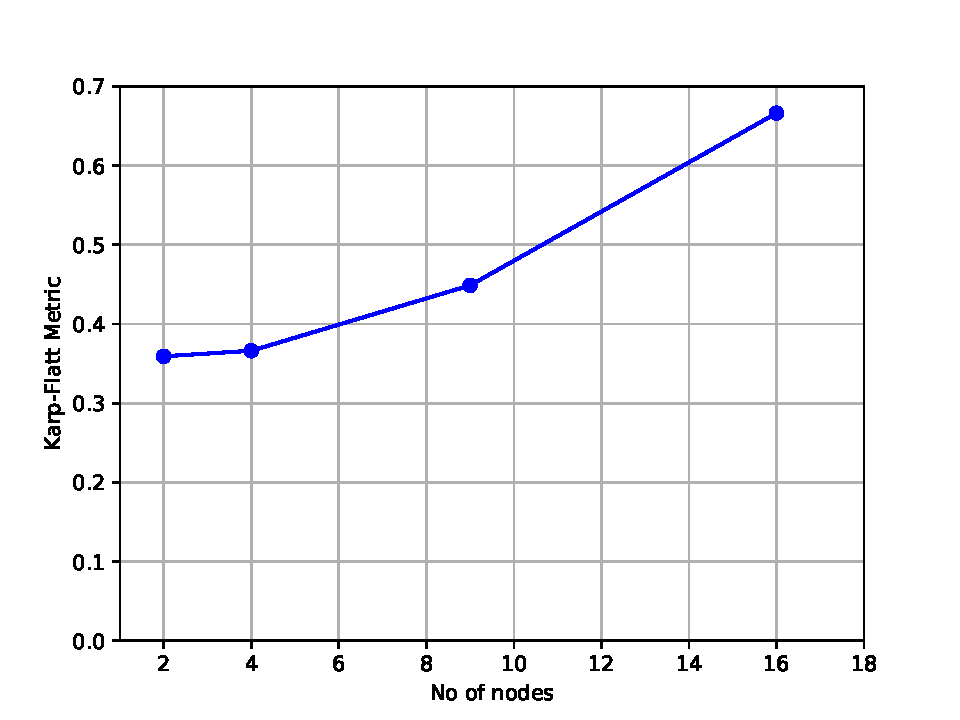
\includegraphics[width=0.5\textwidth]{fig/evals.pdf}
\caption{Karp-Flatt metric for MPI version \label{evals}}
\end{figure}

\subsection{Load Balance}
To get an idea about how much time each worker is waiting for the other workers to finish, we measured the time each worker is taking to write 
its final result to a file. Or in other words this tells how well the data is distributed among the workers. For this we ran the MPI version with 8 nodes (8 workers) and
measured the times each workers is taking to finish its work. The standard deviation of the measured times was 0.0739 seconds which is about 4\% of the average
time consumed by each worker. Therefore we can conclude that we have a reasonable load balance even though we have not implemented techniques for distributing 
the work among the workers fairly.
\section{Performance Bottlenecks and Improvements}
During our evaluation we found several performance bottlenecks. In this section we describe these bottlenecks and how to avoid them in a better implementation.
\begin{itemize}
    \item In our implementation readers are slow because they are fighting over {\em malloc}. As a solution we can malloc block of linked-list nodes each time rather than calling it per node. 
        The synchronization/wait time would be less in this case, but we may end up reserving way more memory than we need, in worst case 99 extra linked-list nodes. 
    \item We found that sequential portion of the parallel execution is very high and also growing with the no of MPI processes. This is due to the fact that we 
        did not exploit all opportunities for parallelism. For example workers do not start the Map-Reduce routine until they receive all the filenames and this
        approach increase the sequential fraction of the program. A better implementation would be to receive filenames in a separate thread and run the Map-Reduce
        alongside it. Unfortunately we did not have time to implement this optimization.
    \item All the workers write their partial results to temporary files and read them back when final results from all the workers are integrated. We did this
        to minimise using locks during parallel execution and decouple the OpenMP and MPI versions for higher portability. This file IO
        operations add a significant overhead. Ideal implementation is to send a specific word to the worker who is responsible for that word right away 
        rather than
        computing the local count for this word and send the result later. We do not know which method is the fastest but it is clear that we have added 
        unnecessary overhead by writing partial results to files.
\end{itemize}
\bibliographystyle{acm}
\bibliography{sample}
\end{document}
